\documentclass[12pt]{article}
\usepackage{import}
\usepackage[scaled]{helvet}
\usepackage[T1]{fontenc}
\renewcommand\familydefault{\sfdefault} 
\usepackage{rotating}
\usepackage{natbib}
\bibliographystyle{agsm} %Imperial College Harvard Style
\usepackage{authblk} %Add second authors and affiliations
\renewcommand{\bibsection}{} %Hide 'References' header
\renewcommand{\abstractname}{Summary}
\usepackage{float}
\usepackage{graphicx}
\usepackage{mathtools}
\usepackage{amsmath}
\usepackage{setspace}
\usepackage[font=singlespacing]{caption}

\usepackage[usenames,dvipsnames, table, xcdraw]{xcolor}
\usepackage{multirow}
\definecolor{mygray}{gray}{0.1}
\definecolor{blue(pigment)}{rgb}{0.2, 0.2, 0.6}
\usepackage[left=2cm,right=2cm,top=2.5cm,bottom=2cm, headheight=15pt]{geometry}
\usepackage{tikz}
\usetikzlibrary{arrows, positioning, shapes.geometric}
\usepackage{hyperref}
\hypersetup{
         colorlinks=true,
         linkcolor=mygray,
         filecolor=magenta,
         urlcolor=mygray,
         citecolor=mygray,}

 %remove chapter text headers
\usepackage{titlesec}
\usepackage{ccaption}

%headers
\usepackage{fancyhdr}

\title{Supplementary Information}
\author{Alberto Scarampi}
\date{May 2024}
\DeclareUnicodeCharacter{2212}{-}
\setcounter{tocdepth}{3}
\setcounter{secnumdepth}{3}

\begin{document}

\maketitle

\tableofcontents


\section{Methyl viologen treatment leads to enhanced light-dependent intracellular ROS accumulation}
Methyl viologen (MV) mediates its cytotoxic effects through the production of reactive oxygen species (ROS). To assess the impact of MV on ROS generation, we employed a ROS quantification assay using cultures of \textit{Synechocystis sp.} PCC 6803 incubated with the ROS-sensitive fluorophore 2',7'-dichlorofluorescein diacetate (DCFH-DA). Given that MV can act as an electron acceptor from Photosystem I (PSI) and its mechanism of action is contingent upon photosynthetic electron flow, the assay was executed under both light and dark conditions. 
In accordance with our hypothesis, cultures treated with 10 $\mu$M MV exhibited a significant intracellular accumulation of ROS. Notably, this ROS accumulation was markedly enhanced under light conditions, thereby corroborating that MV toxicity is mediated via a photosynthetic electron flow-dependent mechanism. 

It is important to note that DCFH-DA is a non-specific ROS indicator, limiting our capacity to differentiate among various ROS types. However, prior studies have demonstrated that MV is capable of generating superoxide anions, hydrogen peroxide, and hydroxyl radicals upon interaction with PSI, both in vitro and in cyanobacterial cells in vivo.

\begin{figure}[H]
    \centering
    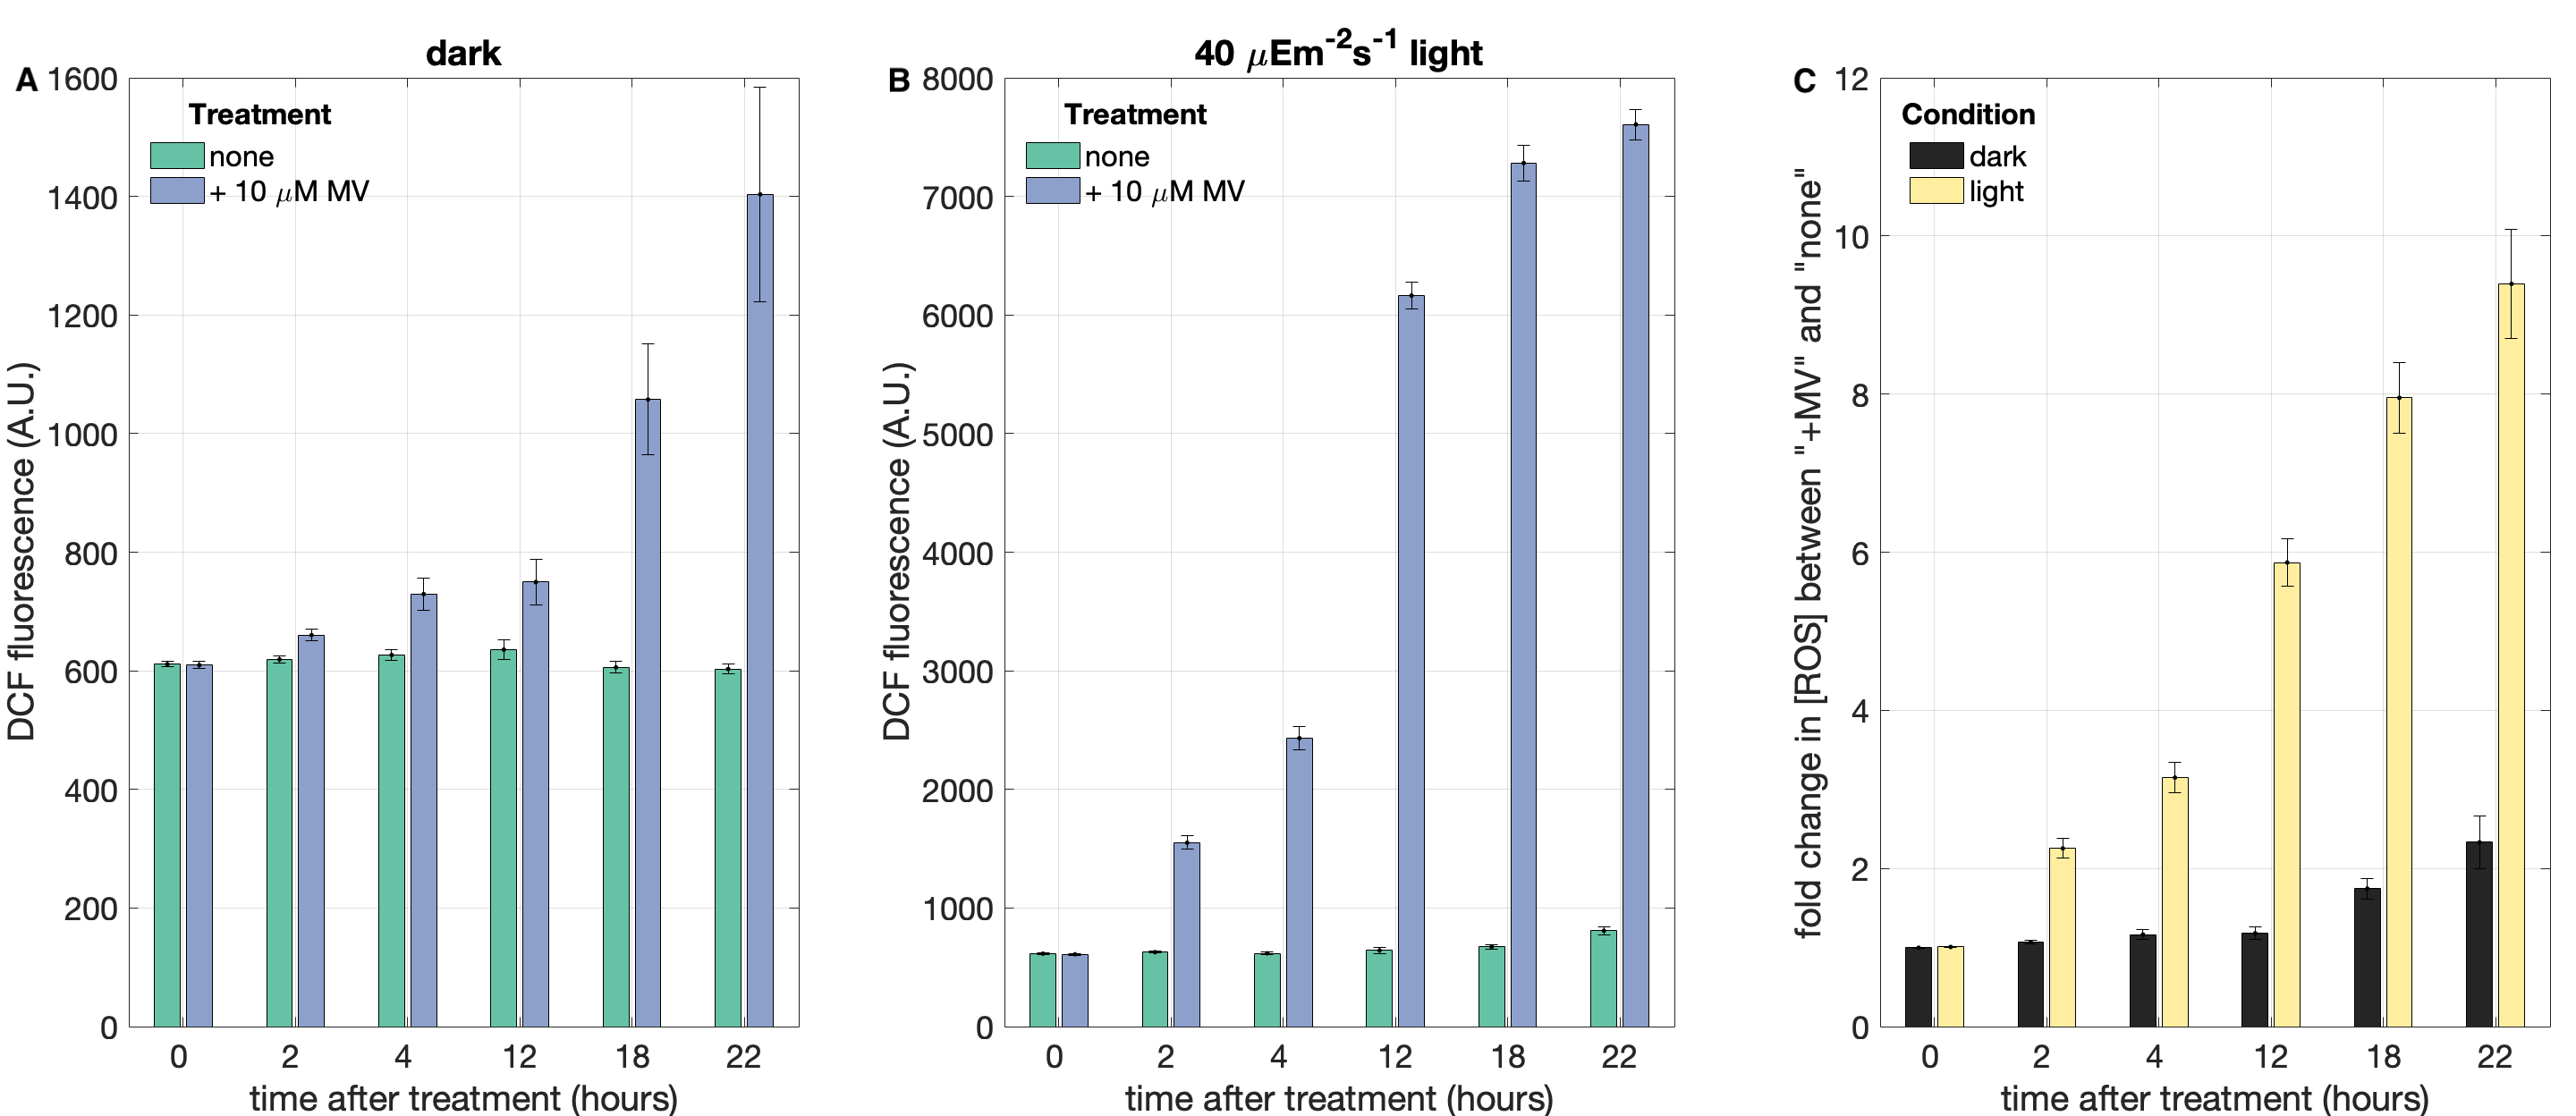
\includegraphics[width=\hsize]{../Figures/MV_adaptation/MV_ROS_DFCDA_Syn6803.png}
    \caption{ROS quantification assay based on the substrate DCFH-DA, which becomes fluorescent upon reaction with intracellular ROS. A) DCF fluorescence in cultures of \textit{Synechocystis} at various time points after treatment with 10 $\mu$M MV (in the dark). B) DCF fluorescence at various time points after treatment with 10 $\mu$M MV (under 40 $\mu$Em$^{-2}$s$^{-1}$ of white light illumination). C) Fold changes in DCF fluorescence between cultures treated with MV and no treatment control in the darkness and light at various time points. Error bars represent standard error of the mean from three biological replicates (individual colonies treated independently).}
    \label{fig:spectraMV1}
\end{figure}

\section{Adaptation to methyl viologen is not due to its abiotic degration over time}
\textit{Synechocystis} cells were able to resume growing after growth-inhibiting treatments with MV. However such growth resumption could have been a result of the abiotic chemical degradation of methyl viologen inside the flasks, especially given that the growth curves were performed for a considerably long time at 30 degrees and in the presence of light. To discard this hypothesis, three cultures from adapted flasks were re-diluted, alongside unadapted controls and their susceptibility against addition of methyl viologen from a freshly prepared stock was quantified in a new growth curve. As demonstrated in Figure \ref{fig:freshstock}, previously adapted cultures were insensitive to addition of fresh methyl viologen, which instead expectedly inhibited the growth of wild-type, "unadapted'' cultures. This confirmd that spontaneous degradation of methyl viologen was not responsible for the observed adaptation, which may be then due to the evolution of biotic resistance mechanisms. 

\begin{figure}[H]
    \centering
    
\includegraphics[width=\hsize]{../Figures/MV_adaptation/growth_curves_firstevolution_Wt_6umMV.png}
    \caption{Growth curves of three independent unadapted (A) and MV-adapted (B) cultures of \textit{Synechocystis sp.} PCC 6803 growing at 30 $\circ$ under constant illumination (intensity = 100 $\mu Em^{-2}s^{-1}$) in the absence (green trace) and upon addition of 6 $\mu M$ of methyl viologen (from a fresh stock) during exponential growth (purple trace). Shaded regions represent standard deviations from three biological replicates.}
    \label{fig:freshstock}
\end{figure}

Figure \ref{fig:spectraMV1} shows the absorbance spectra of unadapted (A) and adapted (B) strains after treatment with methyl viologen after 6 days of growth. Addition of methyl viologen to unadapted strains dramatically altered the pigment content of the strains, resulting in no detectable chlorophyll peaks. On the other hand, adapted strains were able to tolerate fresh addition of methyl viologen. Addition of methyl viologen to these strains results in non-lethal loss of chlorophyll concentration per cell compared to non-treated controls. 

\begin{figure}[H]
    \centering
    
\includegraphics[width=\hsize]{../Figures/MV_adaptation/spectra_endpoint_firstevolution_Wt_6umMV.png}
    \caption{Absorbance spectra of unadapted (A) and adapted (B) cultures of \textit{Synechocystis sp.} PCC 6803 after 6 days of growth at 30 $\circ$ under constant illumination (intensity = 100 $\mu Em^{-2}s^{-1}$) in the absence (green trace) and upon addition  of 6 $\mu M$ of methyl viologen during exponential growth (purple trace). Shaded regions represent standard errors from three biological replicates.}
    \label{fig:spectraMV1}
\end{figure}

\section{Spot plates of Strains Grown in BG11 without or with MV (6 $\mu$M)}
During the spontaneous evolution experiments, the cultures had been growing for over a month and had been exposed to muluiple selective pressures. Therefore in the different flask, different subpopulations could have been present, complicating future DNA sequencing analyses. To overcome this limitations, adapted and unadapted cultures were spotted at different dilutions on BG11 plates containing no or 6 $\mu M$ of methyl viologen. As shown in Figure \ref{fig:spotassayMV}, only previously adapted strains (labelled with "mvR'') were able to survive on methyl viologen containing plates. This allowed to isolate individual colonies, which were then inoculated, grown and their gDNA sent for sequencing.

\begin{figure}[H]
    \centering
    \includegraphics[width=\hsize]{../Figures/MV_adaptation/spotplates_MVadapted_sentforsequencing}
    \caption{Spot plates of 2 unadapted (first two columns on each plates) and 5 adapted (columns 3 to 7) cultures of \textit{Synechocystis sp.} PCC 6803 in BG11 plates without methyl viologen (A) and with the addition of 6 $\mu M$ of methyl viologen (B). Rows correspond to consecutive 10-fold serial dilutions of culture inocula (all starting at on OD750 = 1). Plates were grown at 30 $\circ$ under constant illumination (intensity = 100 $\mu Em^{-2}s^{-1}$) for 10 days.}
    \label{fig:spotassayMV}
\end{figure}

\section{Chronoamperometries strain by strain}

\begin{figure}[H]
    \centering
    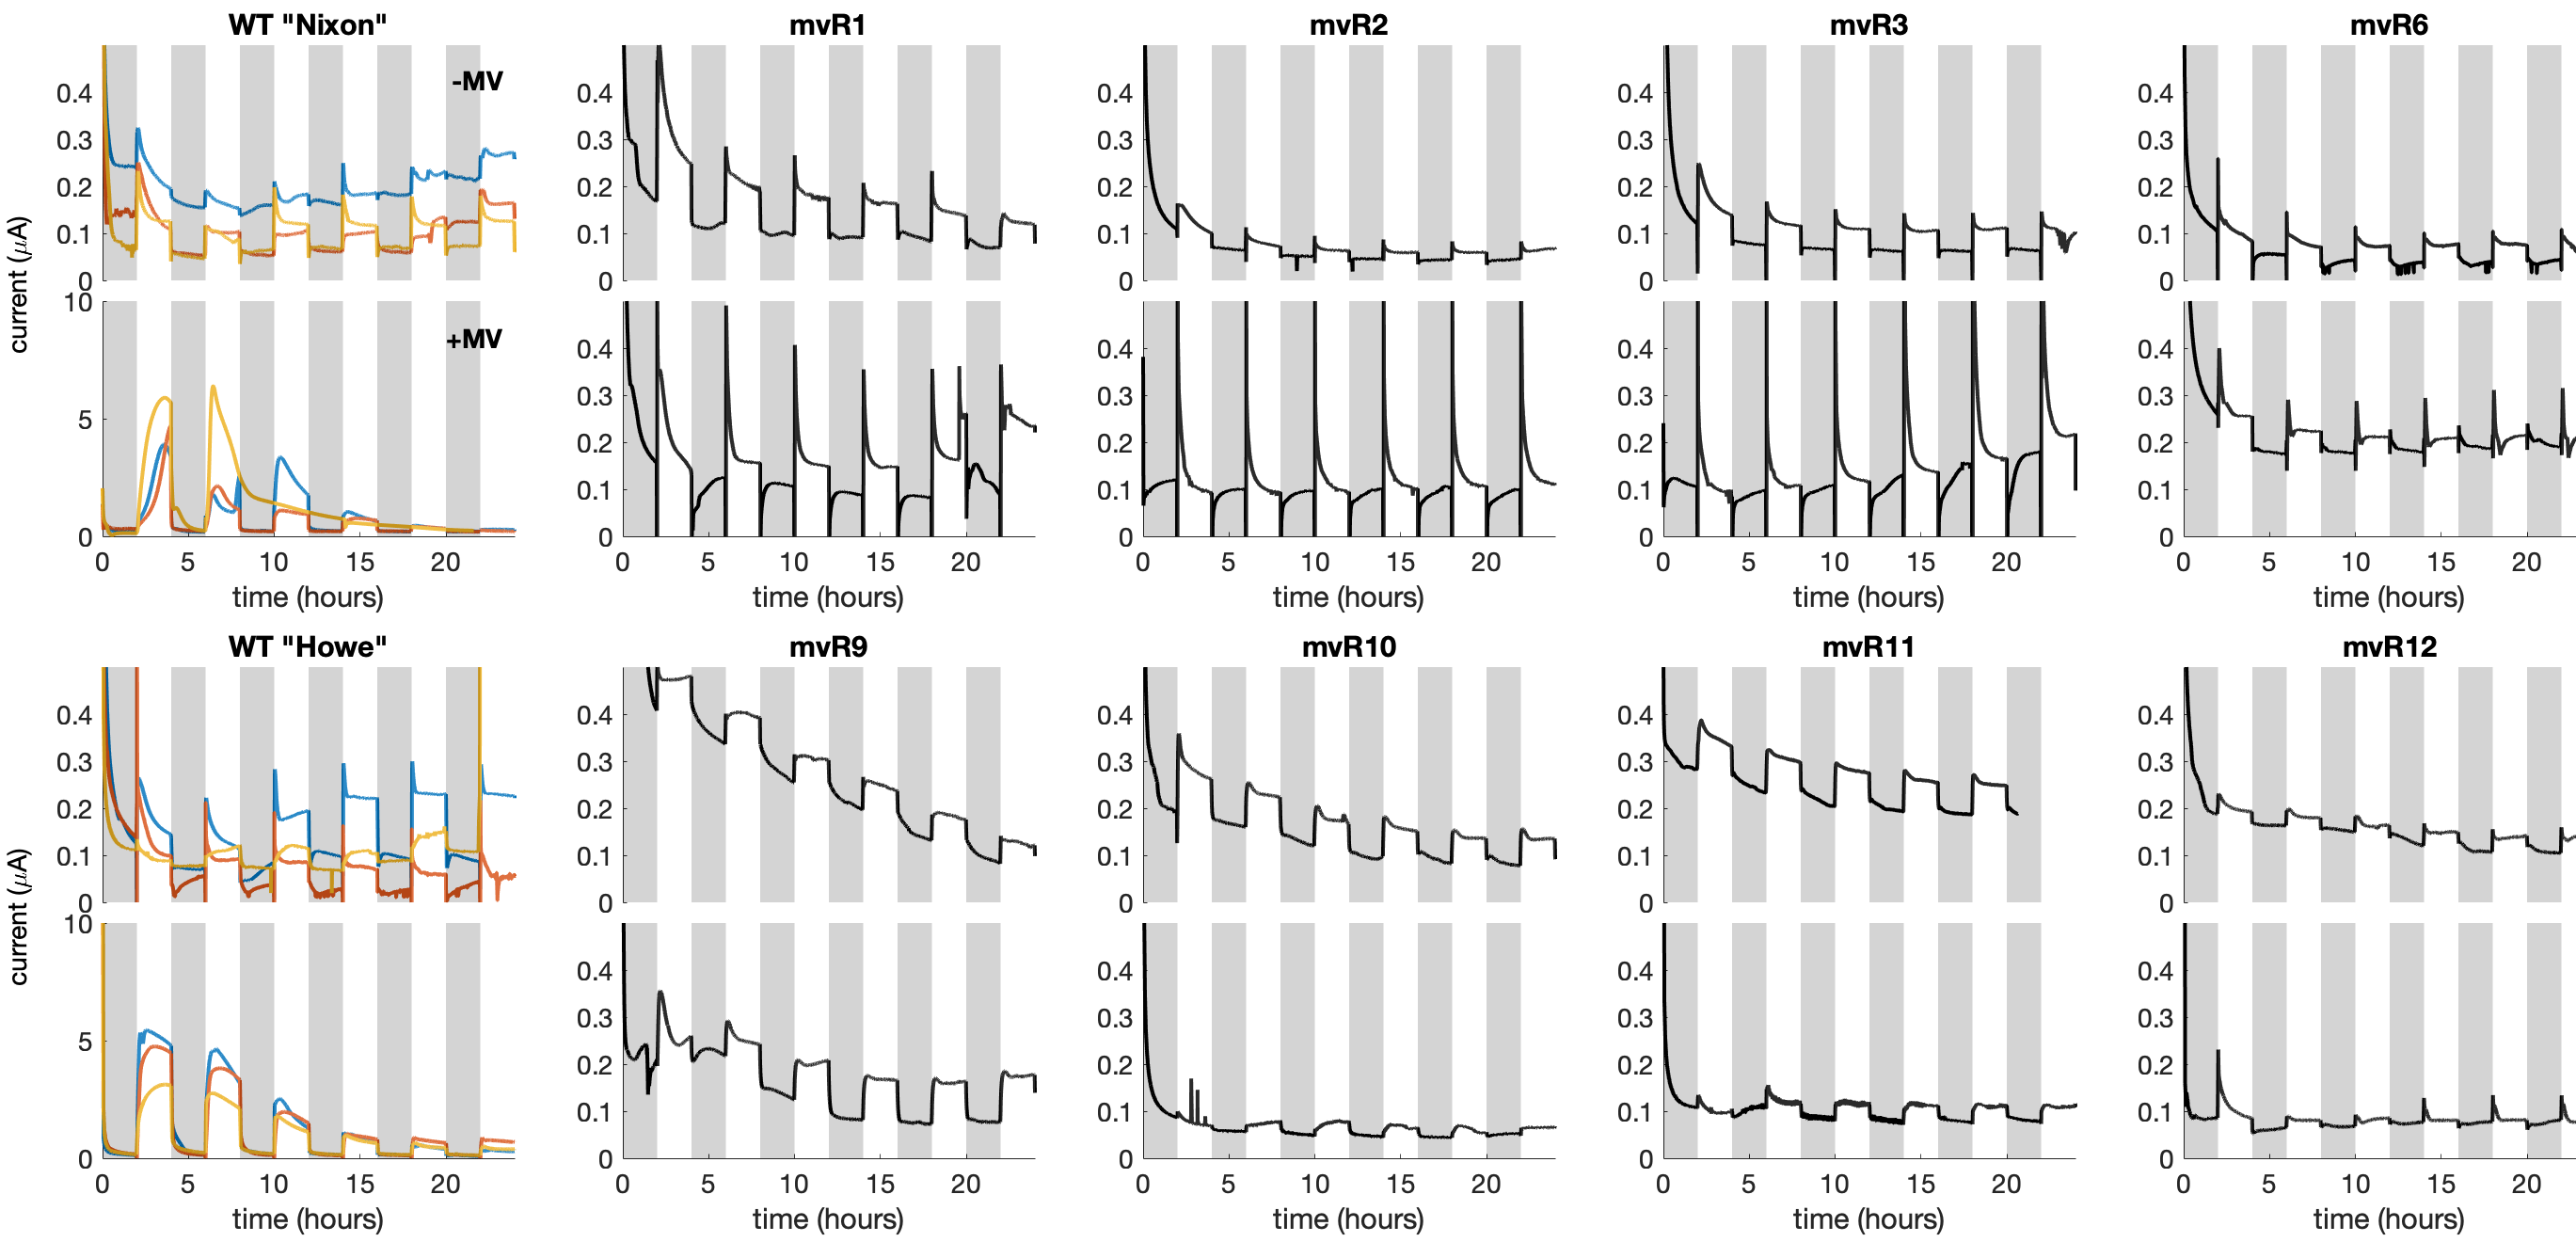
\includegraphics[width=\hsize]{../Figures/MV_adaptation/MVR_chronoamp_panels_all}
    \caption{Chronoamperometry of all strains in the presence (bottom subtiles) and absence of 6 $\mu$M MV. White and gray panels represent periods of illumination and darkness respectively. }
    \label{fig:spotassayMV}
\end{figure}


\section{Quantification of methyl viologen resistance in adapted strains}

The susceptibility of wild-type and resistant strains to varying concentrations of methyl viologen was evaluated by measuring cell density spectrophotometrically over time. Growth rates during the exponential phase were plotted as a function of the methyl viologen concentration for various strains, as depicted in Figure \ref{fig:oxyelectrode}A. A typical inverse sigmoidal relationship was observed between growth rate and methyl viologen concentration, aligning with dose-response expectations typical for an antibiotic agent such as methyl viologen..

The wild-type strains displayed a marked sensitivity to methyl viologen, with growth inhibition observed at concentrations as low as 2 $\mu$M. In contrast, the resistant strains exhibited a notable diversity in their tolerance levels. This might not be surprising, given that each mutant strain evolved its resistance independently, potentially leading to varied underlying genotypic changes and resultant phenotypic manifestations. The half-maximal effective concentration (EC50) values, denoting the concentration of methyl viologen at which the growth rate was reduced by 50$\%$, were derived for each strain. The comparison of these values provided a quantitative metric for resistance (Figure \ref{fig:oxyelectrode}B).
On average, resistant strains showcased an approximate 20-fold increase in tolerance to methyl viologen compared to the wild-type. Remarkably, certain adapted strains (MVR4) displayed almost a 30-fold enhancement in their tolerance limits. Such findings underscore the significant adaptive potential inherent in cyanobacteria and the varied genetic avenues they might employ to counteract the deleterious effects of methyl viologen.

\begin{figure}[H]
    \centering
    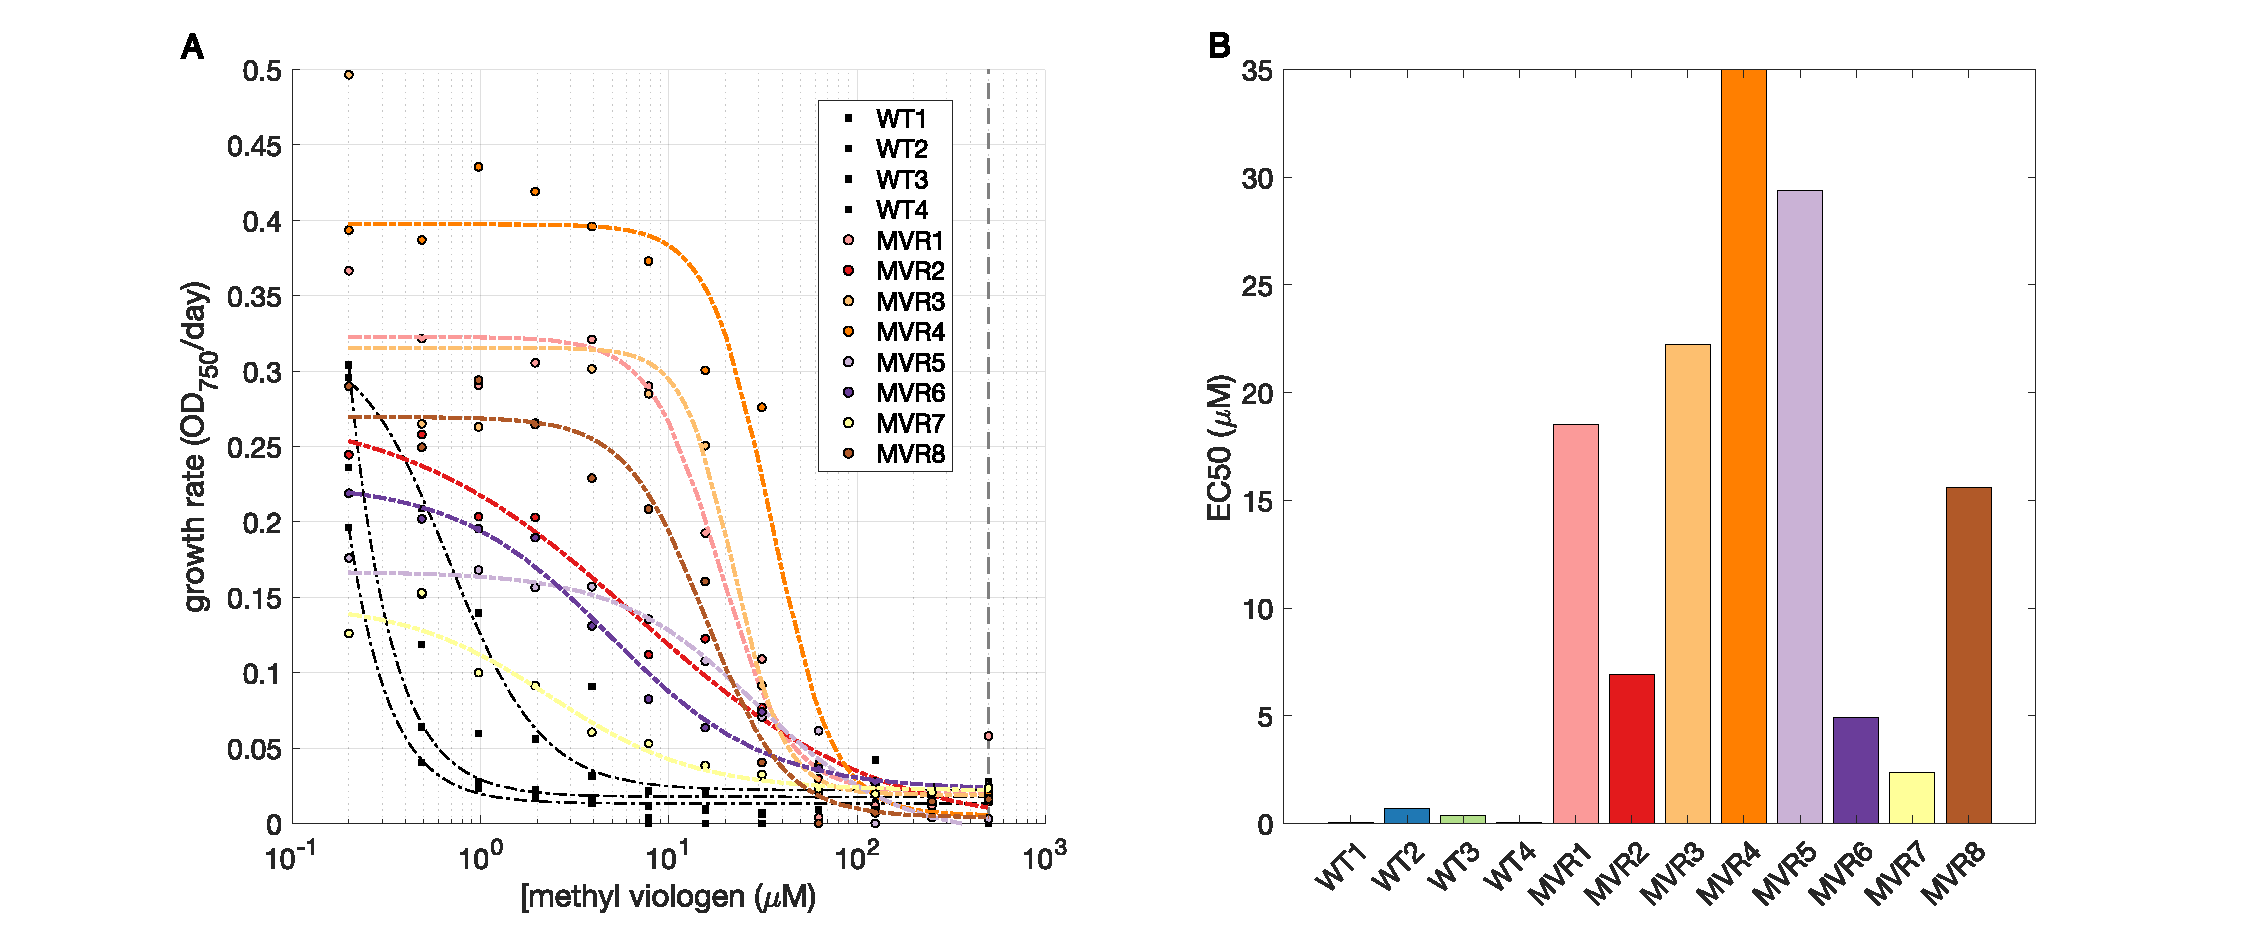
\includegraphics[width=\hsize]{../Figures/MV_adaptation/EC50.pdf}
    \caption{Analysis of growth rate dynamics in the presence of methyl viologen. \textbf{A)} Exponential phase growth rates plotted against methyl viologen concentrations for a range of wild-type and resistant strains. \textbf{B)} The derived half-maximal effective concentrations (EC50) of methyl viologen across different strains, showcasing their respective tolerance levels.}
    \label{fig:oxyelectrode}
\end{figure}


\section{Addition of methyl viologen at various growth phases}

To investigate whether adaptation to methyl viologen depends on the growth stage at which cells are at during the treatment, an additional growth curve was performed during which methyl viologen treatment was added at different cell phases. 
As shown in Figure \ref{fig:MVgrowthstages}, in this case only one culture  managed to adapt to the methyl viologen treatment. This culture was treated during expionential phase.  
The higher the number of cells during the MV treatment, the more likely it would be that in the population there are some resistant cells already which then get enriched. Perhaps what is happening is that during expoential phase, genome replication rate is at its highest and this - together also with the mutagenic effects of the ROS produced by MV - might lead to an enhanced mutation rate in the cells and thus evolution of adapted strains.

\begin{figure}[H]
    \centering
    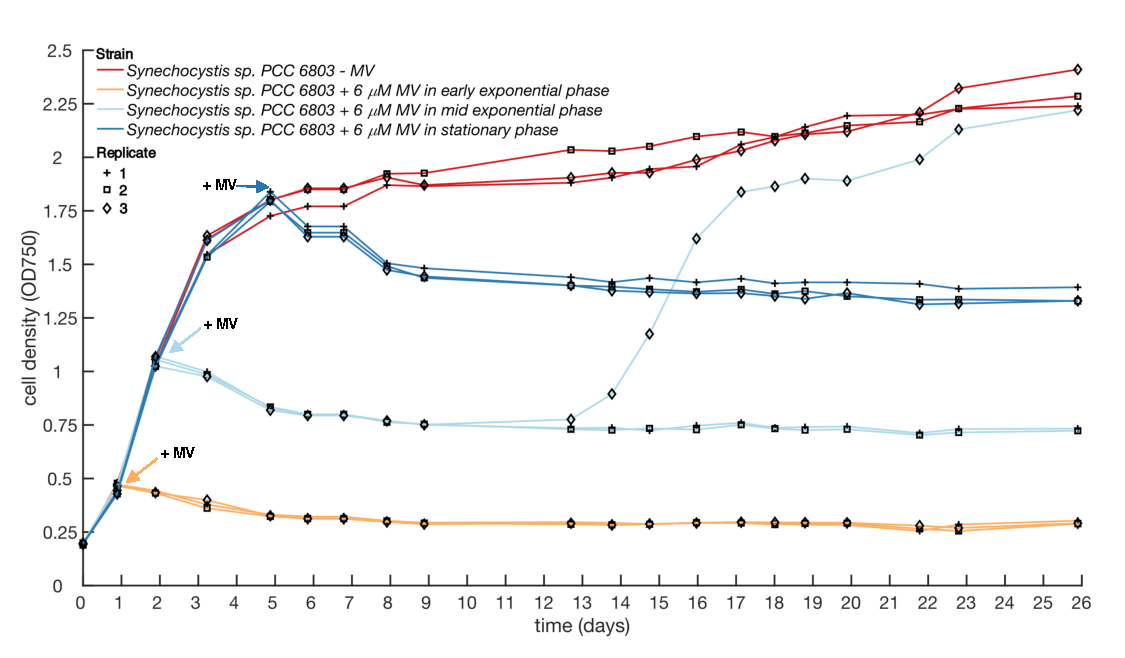
\includegraphics[width=\hsize]{../Figures/MV_adaptation/growthcurves_growthstages_Howe.pdf}
    \caption{Growth curves of \textit{Synechocystis sp.} PCC 6803 strains grown at 30 $\circ$ under constant illumination (intensity = 40 $\mu Em^{-2}s^{-1}$) in the absence (red trace) and upon addition  of 6 $\mu$M of methyl viologen during various growth stages (as indicated by the arrows colored according to the legend on top right).}
    \label{fig:MVgrowthstages}
\end{figure}


\section{PrqA is not essential for spontaneous evolution of MV resistance}

Previous findings have identified that a mutation in the DNA-binding domain of the PrqR repressor led to resistance to methyl viologen. Because PrqR was found to repress the multidrug and toxin extrusion (MATE) protein PrqA, it was suggested that this protein was involded in the detoxification of methyl viologen via extrusion mechanisms. In order to validate whether PrqA is involved in the resistance against methyl viologen, wild-type, mutant and complemented prqA strains were subjected to the same growth profile as above to observe if there were any diffences regarding the spontaneous evolution against methyl viologen for the different strains. 

\begin{figure}[H]
    \centering
    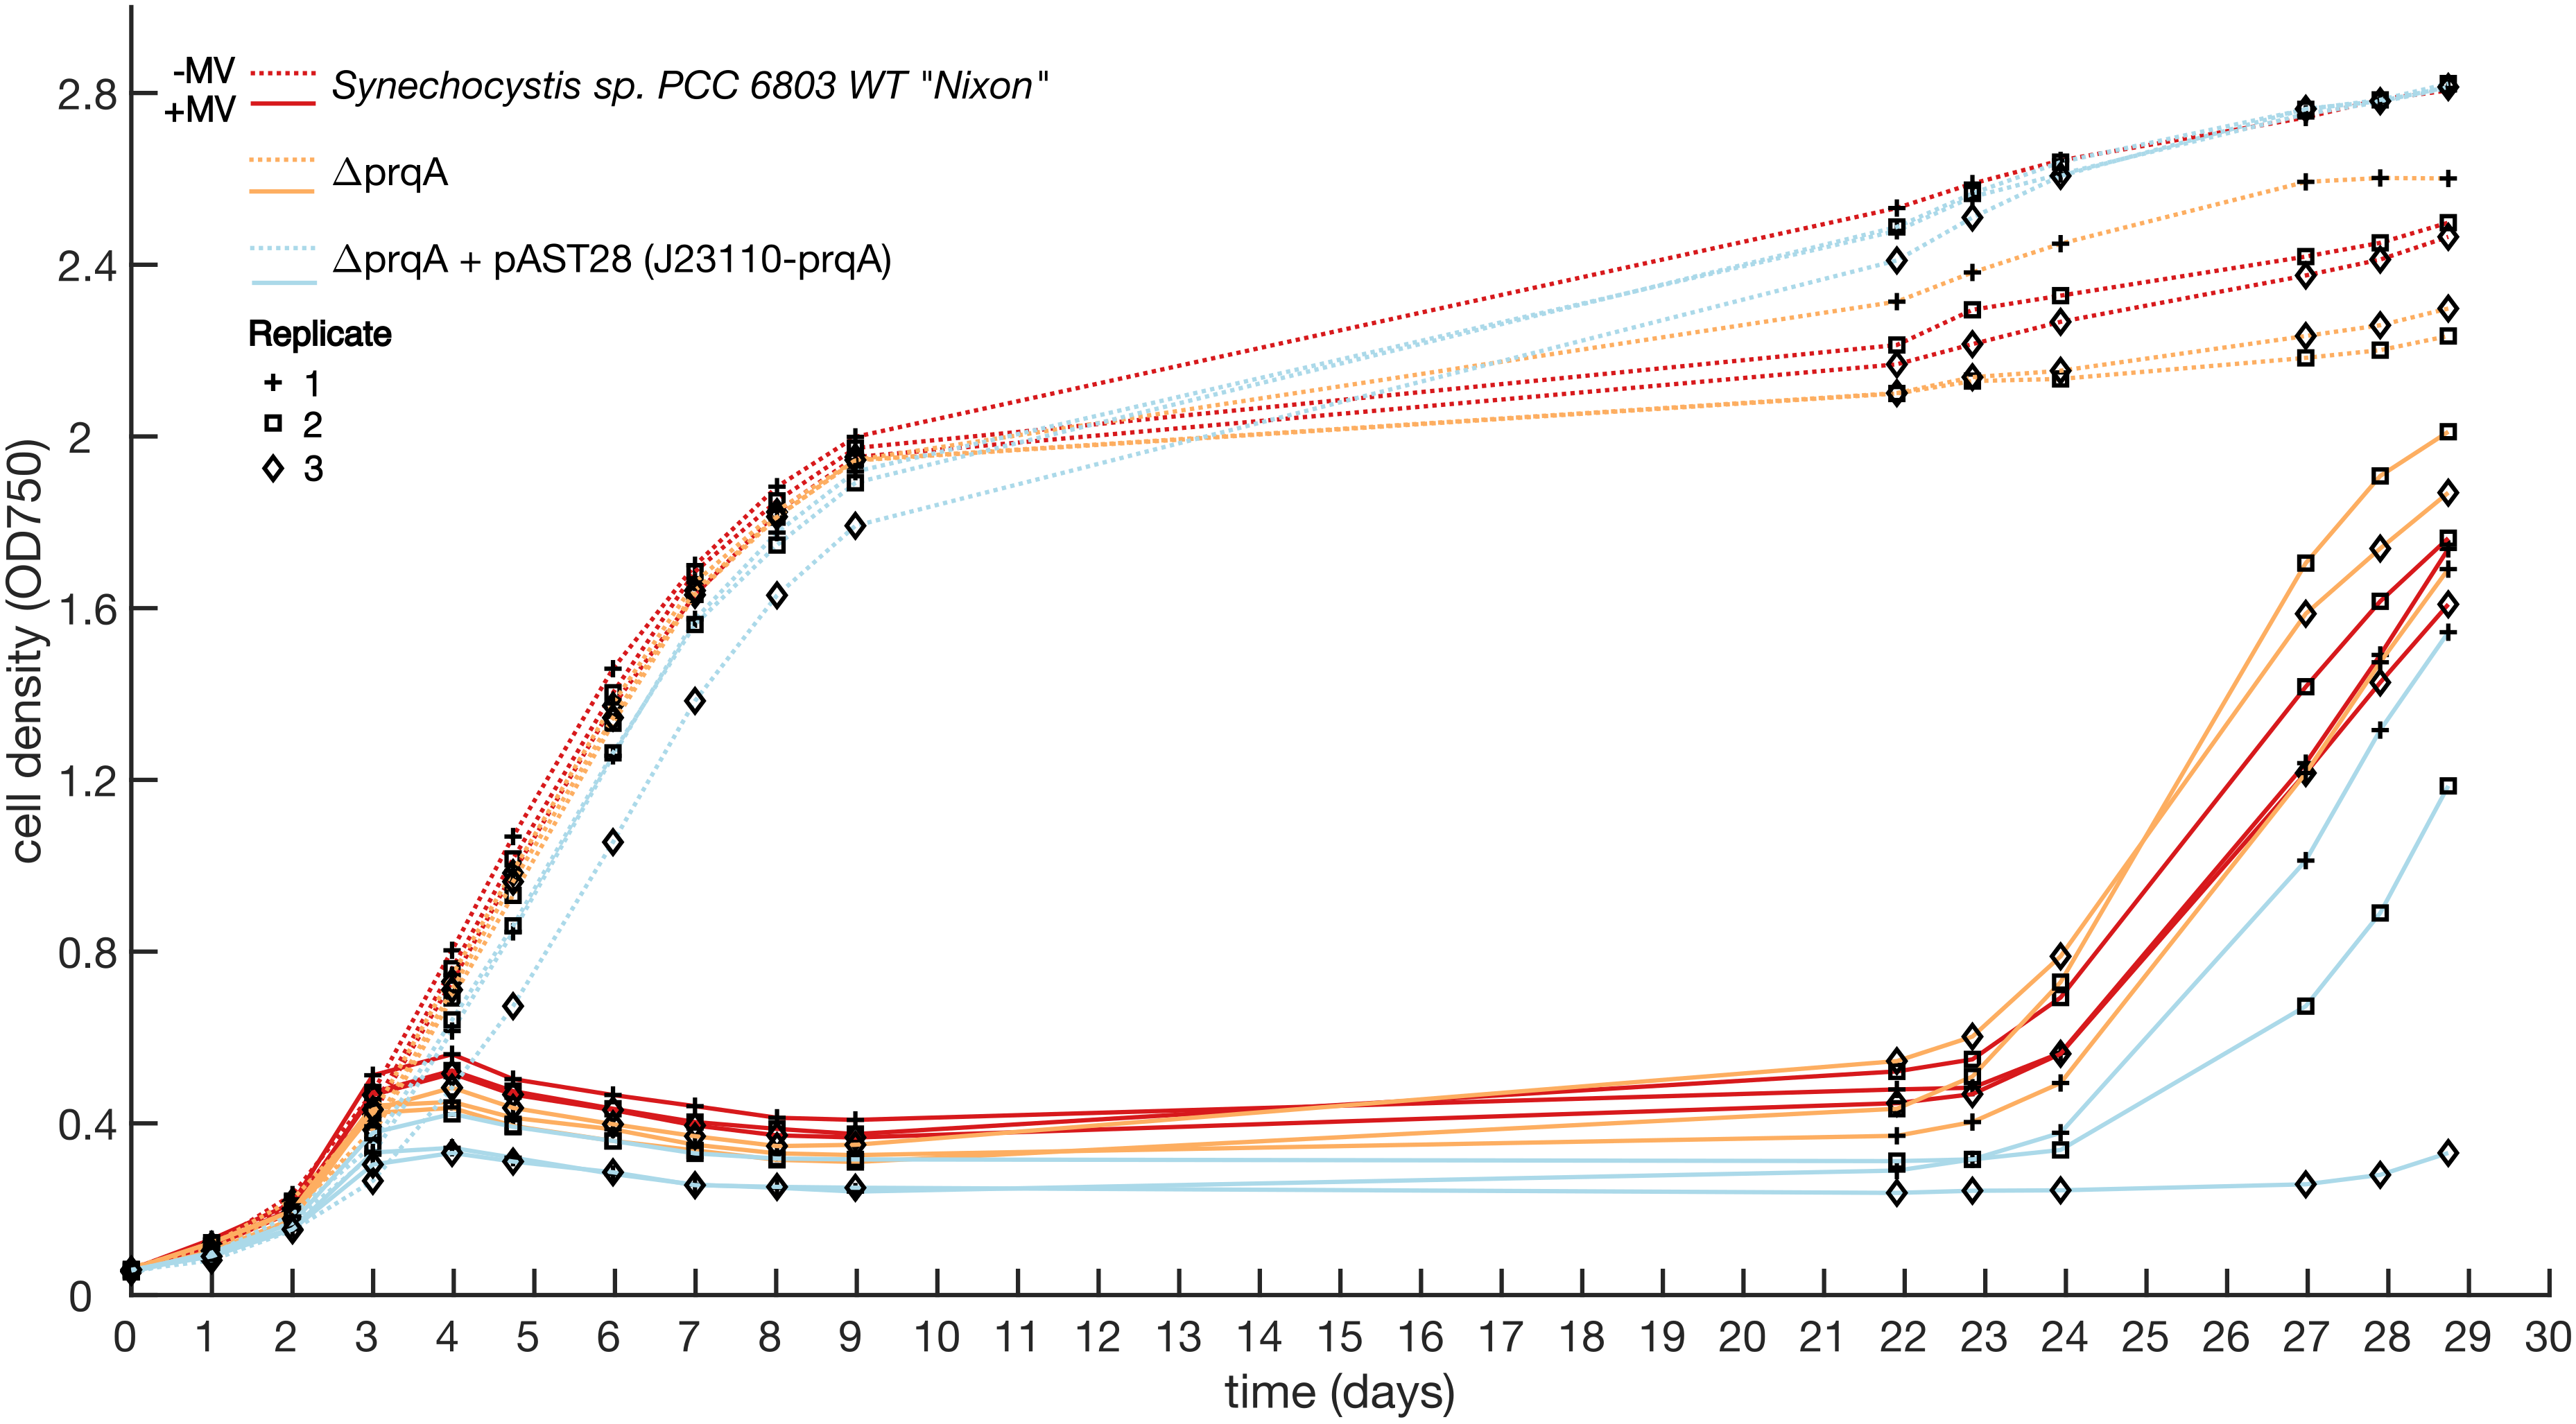
\includegraphics[width=\hsize]{../Figures/MV_adaptation/syn_prqA_MVadapt.png}
    \caption{Growth curves of wild-type, $\Delta$prqA and complemented $\Delta$prqA strains of \textit{Synechocystis sp.} PCC 6803 grown at 30 $\circ$ under constant illumination (intensity = 100 $\mu Em^{-2}s^{-1}$) in the absence (green trace) and upon addition  of 6 $\mu M$ of methyl viologen during exponential growth (purple trace).}
    \label{fig:prqAMV}
\end{figure}

As demonstrated in Figure \ref{fig:prqAMV}, the presence, absence or heterologous expression of PrqA, did not affect the spontaneous evolution of methyl viologen resistance. This suggests that PrqA is not necessary to develop resistance against MV and therefore may not be involved in its extrusion. 


\section{Comparative Genomic Analysis of Wild-Type and Methyl Viologen Resistant Strains}

The genomes of wild-type and MV-resistant \textit{Synechocystis} strains were sequenced to elucidate the genetic determinants potentially underpinning MV resistance. 


\subsection{Genome Sequencing QC Report}

\begin{table}[H]
    \centering
    \begin{tabular}{|c|c|c|c|c|c|c|c|}
    \hline
    \textbf{Sample} & \textbf{\begin{tabular}[c]{@{}c@{}}Concentration \\ (ng/$\mu$l)\end{tabular}} & \textbf{\begin{tabular}[c]{@{}c@{}}Volume \\ ($\mu$l)\end{tabular}} & \textbf{\begin{tabular}[c]{@{}c@{}}Effective \\ (\%)\end{tabular}} & \textbf{\begin{tabular}[c]{@{}c@{}}Error \\ (\%)\end{tabular}} & \textbf{\begin{tabular}[c]{@{}c@{}}Q20 \\ (\%)\end{tabular}} & \textbf{\begin{tabular}[c]{@{}c@{}}Q30 \\ (\%)\end{tabular}} & \textbf{\begin{tabular}[c]{@{}c@{}}GC \\ (\%)\end{tabular}} \\ \hline
    WT\_Nixon & 31.80 & 92 & 99.82 & 0.03 & 97.50 & 92.73 & 55.06 \\ \hline
    WT\_Howe & 27.80 & 98 & 99.78 & 0.03 & 96.75 & 90.99 & 46.50 \\ \hline
    mvR01\_Nixon & 36.40 & 95 & 99.77 & 0.03 & 97.43 & 92.60 & 52.66 \\ \hline
    mvR02\_Nixon & 25.00 & 97 & 99.78 & 0.03 & 97.34 & 92.30 & 47.98 \\ \hline
    mvR03\_Nixon & 30.00 & 101 & 99.81 & 0.03 & 97.65 & 93.02 & 48.64 \\ \hline
    mvR06\_Nixon & 44.60 & 98 & 99.80 & 0.03 & 97.19 & 91.96 & 51.59 \\ \hline
    mvR09\_Howe & 20.60 & 95 & 99.78 & 0.03 & 97.28 & 92.16 & 47.39 \\ \hline
    mvR10\_Howe & 20.20 & 95 & 99.86 & 0.03 & 97.66 & 93.39 & 47.83 \\ \hline
    mvR11\_Howe & 27.80 & 92 & 99.87 & 0.03 & 97.55 & 93.14 & 46.53 \\ \hline
    mvR12\_Howe & 19.60 & 98 & 99.86 & 0.03 & 97.65 & 93.31 & 47.50 \\ \hline
    \end{tabular}
\end{table}

Alignment of the trimmed and paired reads from whole genome sequencing experiments was carried out against several reference genome sequences of \textit{Synechocystis} substrains (Figures \ref{fig:WTN_NC000911} and \ref{fig:WTN_NC000911}). \ref{fig:SNPs} shows the results of the type and number of mutations of both wild types as compared to all \textit{Synechocystis} substrain reference genomes available in the NCBI datatase. For both wild-types, the GT-Kazusa reference genome was the one that resulted in the least amount of SNPs.

\begin{figure}[H]
    \centering
    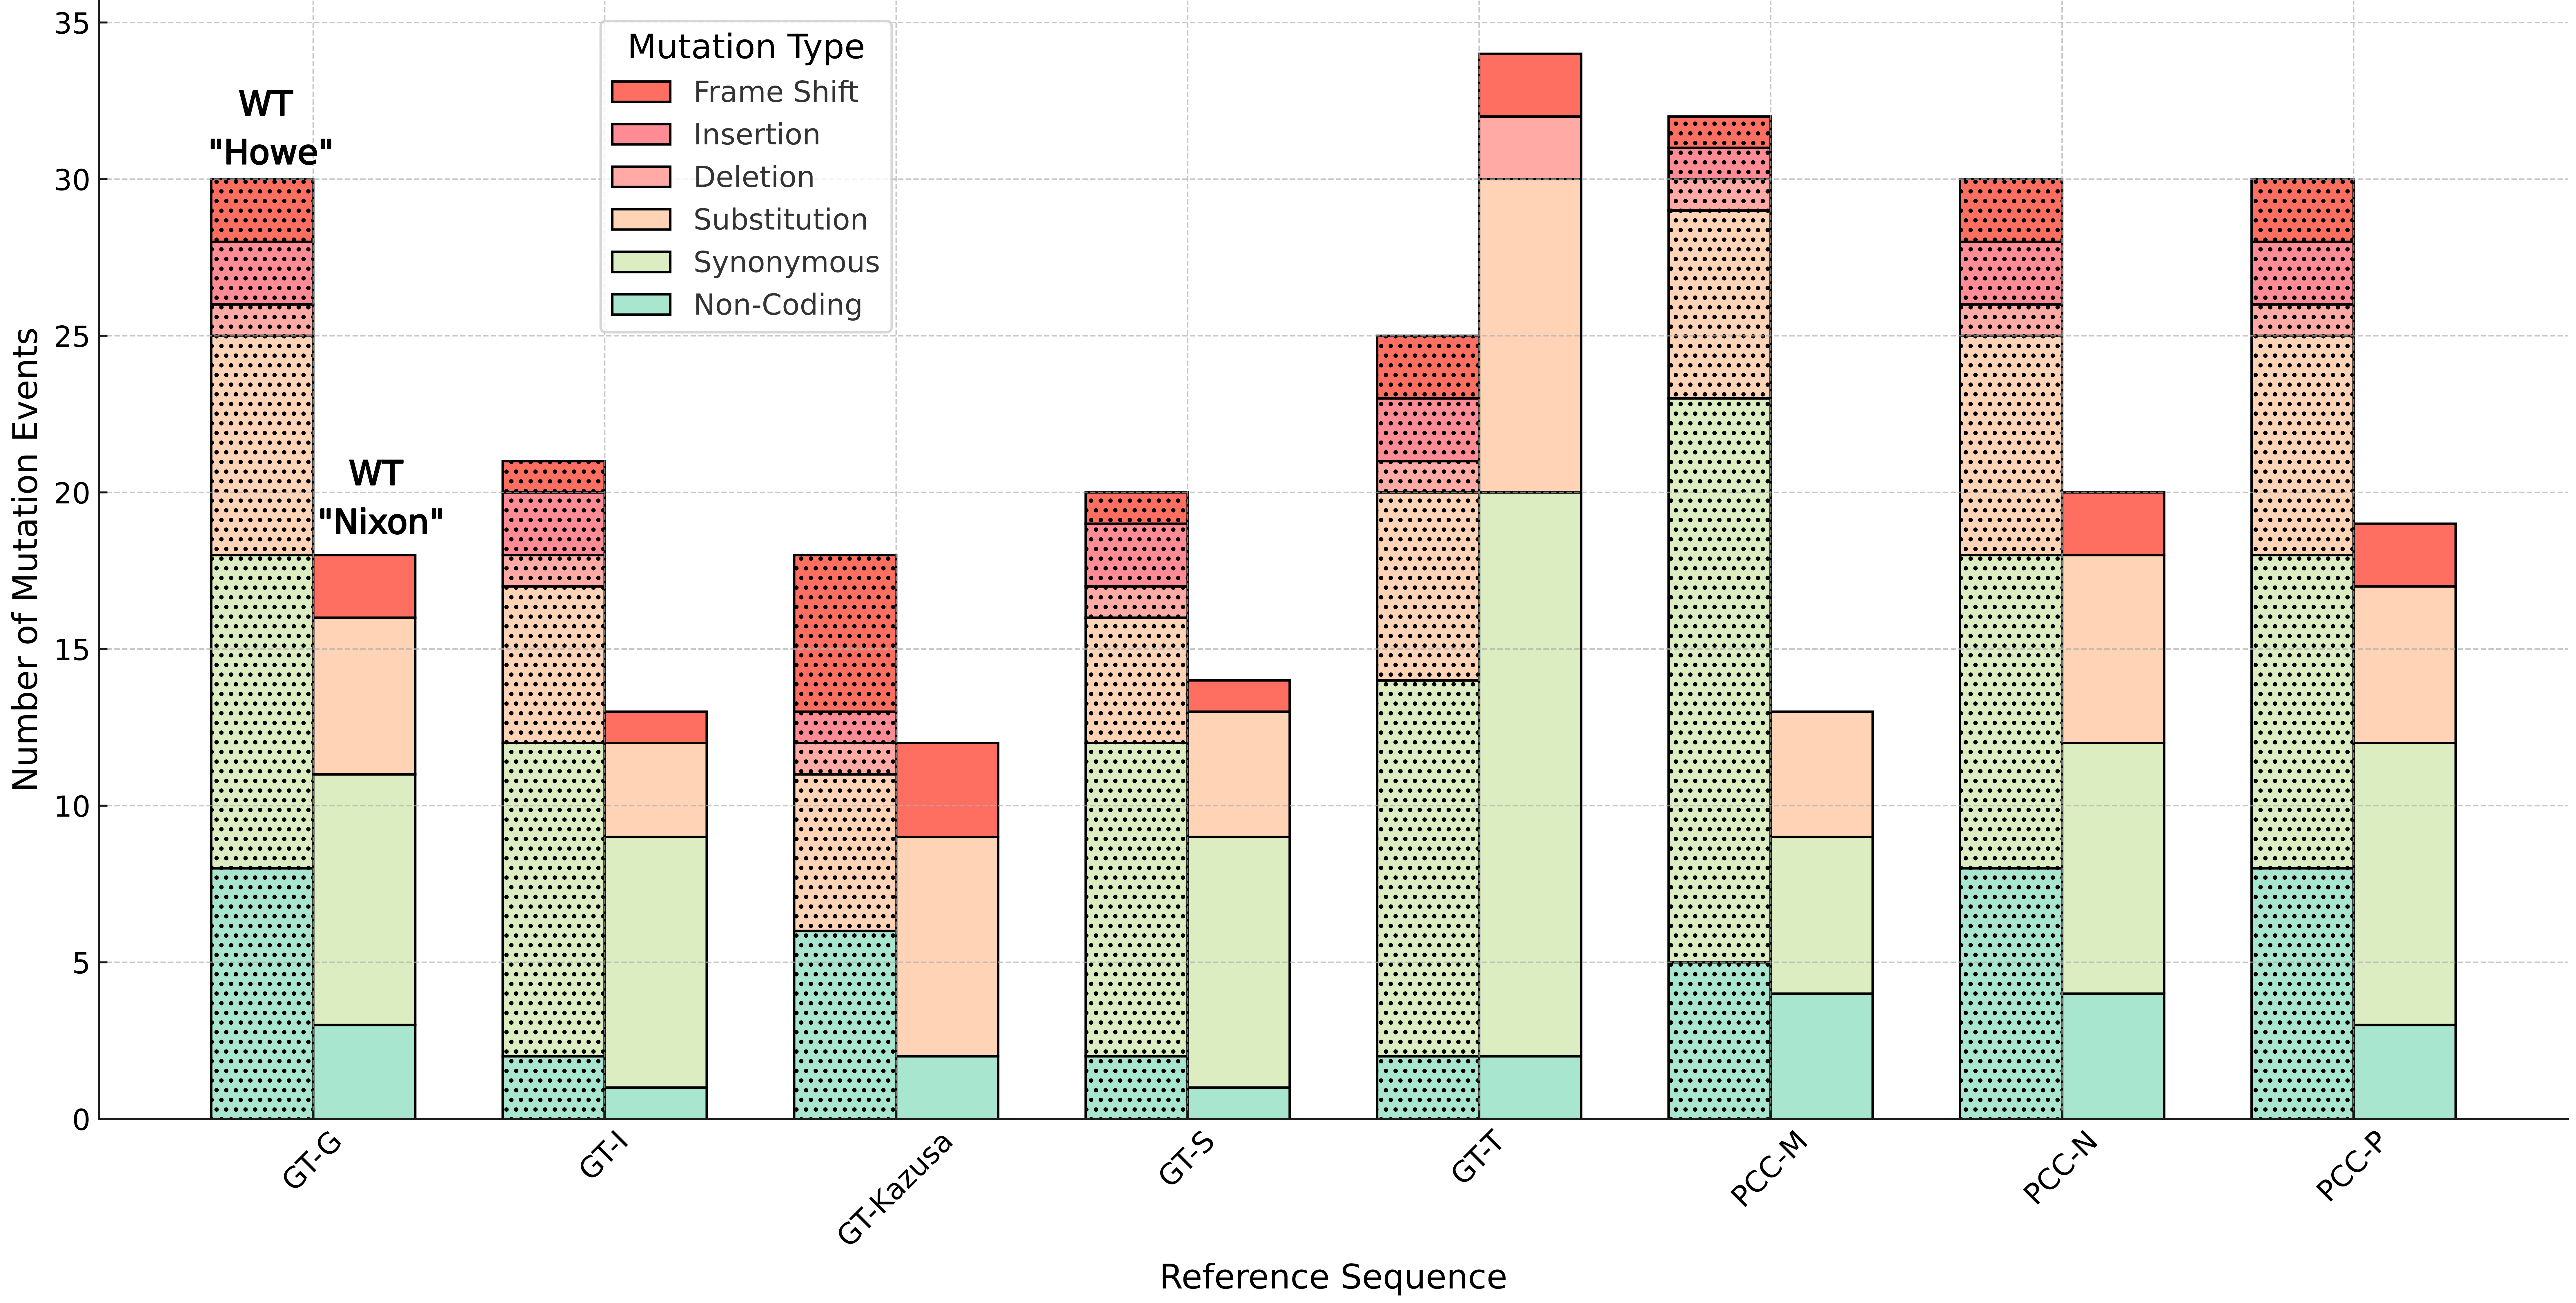
\includegraphics[width=\hsize]{../Figures/MV_adaptation/mutation_events_plot.png}
    \caption{Overview of the variant analysis results.}
    \label{fig:SNPs}
\end{figure}

The mutations were then filtered to identify only non-synonymous ones which results in mutated proteins. 

\begin{figure}[H]
    \centering
    \includegraphics[width=\hsize]{../Figures/WGS/wt_Nixon_vs_NC000911_genomeview.png}
    \caption{Trimmed and paired reads from whole genome sequencing experiments of \textit{Synechocystis} "Nixon'' wild-type aligned to reference "Kazusa'' strain (NC000911). Numbered are mutation events found within coding sequences of the reference genome.}
    \label{fig:WTN_NC000911}
\end{figure}

For both wild-type strains, the aligned reads covered 100$\%$ of the reference genome sequences, indicating that the genomic sequencing was succesfull.
Approximately 20 mutations in coding regions were identified for both the Howe and Nixon wild-type strains. Many mutations were found in transposases, which is unsurprising given the highly evolvable nature of these mobile genetic elements. Many mutations also had moderately small variant frequencies values, indicating that such mutationswere either artifacts of sequencing or not fully segregated mutations. Cyanobacteria, have a high degree of poliploidy in their genomes so this might explain why.


\begin{figure}[H]
    \centering
    \includegraphics[width=\hsize]{../Figures/WGS/wt_Howe_vs_NC000911_genomeview.png}
    \caption{Trimmed and paired reads from whole genome sequencing experiments of \textit{Synechocystis} "Howe'' wild-type aligned to reference "Kazusa'' strain (NC000911). Numbered are mutation events found within coding sequences of the reference genome.}
    \label{fig:WTH_NC000911}
\end{figure}

The Nixon wild-type strain appeared to have a mutation in the type II secretion system F family protein (pilC). Such mutation corresponded to a  deletion from (G)9 to (G)8, leading to a Frame Shift. Such mutation has been identified previously as an artefact due to repetitive G nucleotides and misannotations in the database. Analogously, the Howe substrain exhibited an - at first surprising -  substitution in photosystem I. Such mutation has also been identified previously as a misannotation of the reference genome sequence NC000911. In order to identify genotypic differences between the "Howe'' and "Nixon'' substrains, all variants identified were filtered to retain only the ones that were unique between the two substrains. This was performed for each of the reference sequence that the reads were aligned to. The analysis revealed that both strains have mutations in transposase genes, suggesting potential genomic instability or changes in the frequency of genomic rearrangements.
"Nixon" has mutations affecting sugar transport and secretion systems, potentially altering its carbohydrate metabolism and interactions with the environment.
"Howe" has mutations affecting motility and respiratory processes, suggesting potential changes in movement and energy metabolism.

    \begin{table}[H]
        \centering
        \tiny	
        \begin{tabular}{c|c|c|c|c|c|c|c|c|}
        \cline{2-9}
        & \textbf{Gene} & \textbf{Product} & \begin{tabular}[c]{@{}c@{}}\textbf{CDS} \\ \textbf{Position}\end{tabular} & \textbf{Change} & \begin{tabular}[c]{@{}c@{}}\textbf{Protein} \\ \textbf{Effect}\end{tabular} & \begin{tabular}[c]{@{}c@{}}\textbf{Amino} \\ \textbf{Acid Change}\end{tabular} & \begin{tabular}[c]{@{}c@{}}\textbf{Variant} \\ \textbf{Frequency}\end{tabular} & \textbf{Reference} \\ \hline
        \multicolumn{1}{|c|}{1} & sll0020 & \begin{tabular}[c]{@{}c@{}}ATP-dependent  Clp protease \\ ATP-binding subunit\end{tabular} & 580 & T   -> G & Substitution & K   -> Q & 0.997 & GT-T \\ \hline
        \multicolumn{1}{|c|}{2} & sll0401 & citrate synthase & 434 & A -> C & Substitution & M -> R & 1 & PCC-M \\ \hline
        \multicolumn{1}{|c|}{3} & sll0414 & DUF4335   domain-containing protein & 334 & +C & Frame   Shift &  & 0.955 & GT-Kazusa \\ \hline
        \multicolumn{1}{|c|}{4} & sll0761 & hypothetical protein & 302 & -C & Frame Shift &  & 0.952 & GT-Kazusa \\ \hline
        \multicolumn{1}{|c|}{5} & sll0762 & Ig-like   domain-containing protein & 8924 & +C & Frame   Shift &  & 0.957 & GT-Kazusa \\ \hline
        \multicolumn{1}{|c|}{6} & sll0771 & sugar porter family MFS transporter & 85 & (C)8 -> (C)7 & Frame Shift &  & 0.919 & GT-T \\ \hline
        \multicolumn{1}{|c|}{7} & sll0789 & \begin{tabular}[c]{@{}c@{}}two-component   \\ system regulator RppA\end{tabular} & 403 & CCA   -> TCG & Substitution & W   -> R & \begin{tabular}[c]{@{}c@{}}0.517   \\ +- 0.003\end{tabular} & \begin{tabular}[c]{@{}c@{}}GT-Kazusa,  GT-I, GT-S, \\ GT-T, PCC-N, PCC-P, GT-G\end{tabular} \\ \hline
        \multicolumn{1}{|c|}{8} & sll0789 & \begin{tabular}[c]{@{}c@{}}two-component \\ system regulator RppA\end{tabular} & 397 & TTG -> GTC & Substitution & Q -> D & \begin{tabular}[c]{@{}c@{}}0.550\\  +- 0.0005\end{tabular} & \begin{tabular}[c]{@{}c@{}}GT-Kazusa, PCC-P, PCC-N, \\ GT-T, GT-S, GT-I, GT-G\end{tabular} \\ \hline
        \multicolumn{1}{|c|}{9} & sll0798 & sensor   histidine kinase RppB & 1339 & A   -> C & Substitution & F   -> V & 0.501 & PCC-M \\ \hline
        \multicolumn{1}{|c|}{10} & sll0798 & sensor histidine kinase RppB & 1336 & T -> G & Substitution & I -> L & 0.516 & PCC-M \\ \hline
        \multicolumn{1}{|c|}{11} & sll1201 & Rpn  family nuclease/putative transposase & 340 & C   -> A & Substitution & V   -> L & 0.509 & PCC-M \\ \hline
        \multicolumn{1}{|c|}{12} & sll1389 & hypothetical protein & 430 & (G)8 -> (G)7 & Frame Shift &  & \begin{tabular}[c]{@{}c@{}}0.89 +- \\ 0.012\end{tabular} & \begin{tabular}[c]{@{}c@{}}GT-Kazusa, PCC-P, PCC-N, \\ PCC-M, GT-T,  GT-S, GT-I, GT-G\end{tabular} \\ \hline
        \multicolumn{1}{|c|}{13} & sll1575 & serine/threonine-protein  kinase & 308 & +T & Frame   Shift &  & \begin{tabular}[c]{@{}c@{}}0.972   \\ +- 0\end{tabular} & PCC-N,  PCC-P \\ \hline
        \multicolumn{1}{|c|}{14} & sll1732 & \begin{tabular}[c]{@{}c@{}}NAD(P)H-quinone oxidoreductase \\ subunit F\end{tabular} & 1766 & C -> T & Substitution & R -> Q & 0.997 & GT-T \\ \hline
        \multicolumn{1}{|c|}{15} & sll1895 & EAL   domain-containing protein & 1134 & (T)3   -> (T)2 & Frame   Shift &  & 0.965 & GT-G \\ \hline
        \multicolumn{1}{|c|}{16} & sll1968 & anti-sigma regulatory factor & 124 & T -> C & Substitution & K -> E & 1 & GT-I \\ \hline
        \multicolumn{1}{|c|}{17} & slr0162 & type   II secretion system F protein & 420 & (G)9   -> (G)8 & Frame   Shift &  & 0.835 & GT-Kazusa \\ \hline
        \multicolumn{1}{|c|}{18} & slr0168 & DUF4114 domain-containing protein & 1207 & A -> G & Substitution & K -> E & 1 & GT-Kazusa \\ \hline
        \multicolumn{1}{|c|}{19} & slr0611 & solanesyl   diphosphate synthase & 205 & +ACGGCG & Insertion & -> TA & \begin{tabular}[c]{@{}c@{}}0.554   \\ +- 0\end{tabular} & \begin{tabular}[c]{@{}c@{}}GT-G,  GT-I, GT-S, \\ GT-T, PCC-N, PCC-P\end{tabular} \\ \hline
        \multicolumn{1}{|c|}{20} & slr0665 & bifunctional aconitate hydratase & 31 & G -> A & Substitution & D -> N & \begin{tabular}[c]{@{}c@{}}0.515 \\ +- 0\end{tabular} & \begin{tabular}[c]{@{}c@{}}GT-Kazusa, PCC-P, PCC-N, \\ GT-T, GT-S,  GT-I, GT-G\end{tabular} \\ \hline
        \multicolumn{1}{|c|}{21} & slr0665 & bifunctional   aconitate hydratase & 26 & T   -> C & Substitution & V   -> A & \begin{tabular}[c]{@{}c@{}}0.518   \\ +- 0\end{tabular} & \begin{tabular}[c]{@{}c@{}}GT-Kazusa,  PCC-P, PCC-N, \\ GT-T, GT-S, GT-I, GT-G\end{tabular} \\ \hline
        \multicolumn{1}{|c|}{22} & slr0667 & IS5 family transposase & 443 & +CATGGA & Insertion & G -> VHG & \begin{tabular}[c]{@{}c@{}}0.836 \\ +- 0.01\end{tabular} & \begin{tabular}[c]{@{}c@{}}GT-Kazusa, PCC-P, PCC-N, \\ PCC-M, GT-T,  GT-S, GT-I, GT-G\end{tabular} \\ \hline
        \multicolumn{1}{|c|}{23} & slr1085 & glycosyltransferase  family 4 protein & 67 & \begin{tabular}[c]{@{}c@{}}-GAACT\\ GTCCATC\end{tabular} & Deletion & ELSI   -> & \begin{tabular}[c]{@{}c@{}}0.74   \\ +- 0.043\end{tabular} & \begin{tabular}[c]{@{}c@{}}GT-Kazusa,  PCC-P, PCC-N, \\ PCC-M, GT-T, GT-S, GT-I, GT-G\end{tabular} \\ \hline
        \multicolumn{1}{|c|}{24} & slr2031 & \begin{tabular}[c]{@{}c@{}}PP2C family protein-serine/threonine \\ phosphatase\end{tabular} & 25 & A -> T & Substitution & S -> C & 1 +- 0 & GT-G, PCC-N, PCC-P \\ \hline
        \multicolumn{1}{|c|}{25} & slr2031 & \begin{tabular}[c]{@{}c@{}}PP2C family protein-serine/threonine \\ phosphatase\end{tabular} & 27 & CTT   -> AAA & Substitution & SL   -> RK & \begin{tabular}[c]{@{}c@{}}0.645   \\ +- 0.005\end{tabular} & GT-G \\ \hline
        \multicolumn{1}{|c|}{26} & slr2031 & \begin{tabular}[c]{@{}c@{}}PP2C family protein-serine/threonine  \\ phosphatase\end{tabular} & 42 & T -> A & Substitution & D -> E & \begin{tabular}[c]{@{}c@{}}0.6 \\ +- 0\end{tabular} & GT-G, PCC-N, PCC-P \\ \hline
        \multicolumn{1}{|c|}{27} & slr2122 & acylneuraminate cytidylyltransferase & 318 & C   -> G & Substitution & S   -> R & 1 & PCC-M \\ \hline
        \multicolumn{1}{|c|}{28} & ssl2749 & nucleotidyltransferase family protein & 74 & T -> C & Substitution & Q -> R & 0.534 & PCC-M \\ \hline
        \end{tabular}
        \label{Tab:NixMut}
        \caption{Unique mutations found in WT "Nixon''}
    \end{table}

Interestingly the "Nixon'' substrains harbours a deletion in the glycosyltransferase family 4 protein, and a frame shift in the sugar porter family MFS transporter protein (sll0771).

    \begin{table}[H]
        \centering
        \tiny	
        \begin{tabular}{c|c|c|c|c|c|c|c|c|}
        \cline{2-9}
         & \textbf{Gene} & \textbf{Product} & \begin{tabular}[c]{@{}c@{}}\textbf{CDS} \\ \textbf{Position}\end{tabular} & \textbf{Change} & \begin{tabular}[c]{@{}c@{}}\textbf{Protein} \\ \textbf{Effect}\end{tabular} & \begin{tabular}[c]{@{}c@{}}\textbf{Amino Acid} \\ \textbf{Change}\end{tabular} & \begin{tabular}[c]{@{}c@{}}\textbf{Variant} \\ \textbf{Frequency}\end{tabular} & \textbf{Reference} \\ \hline
        \multicolumn{1}{|c|}{1} & sll0092 & transposase & 232 & A   -> G & Substitution & Y   -> H & \begin{tabular}[c]{@{}c@{}}0.557\\ +- 0\end{tabular} & \begin{tabular}[c]{@{}c@{}}GT-Kazusa, PCC-P, PCC-N, \\ GT-T, GT-S, GT-I, GT-G\end{tabular} \\ \hline
        \multicolumn{1}{|c|}{2} & sll0092 & transposase & 205 & G -> A & Substitution & P -> S & \begin{tabular}[c]{@{}c@{}}0.523 \\ +- 0\end{tabular} & GT-Kazusa, GT-G, GT-I \\ \hline
        \multicolumn{1}{|c|}{3} & sll0092 & transposase & 269 & T   -> C & Extension &  & \begin{tabular}[c]{@{}c@{}}0.614\\ +- 0\end{tabular} & \begin{tabular}[c]{@{}c@{}}GT-Kazusa, PCC-P, PCC-N, \\ GT-T, GT-S, GT-I, GT-G\end{tabular} \\ \hline
        \multicolumn{1}{|c|}{4} & sll0762 & hypothetical protein & 302 & -C & Frame Shift &  & 0.928 & GT-Kazusa \\ \hline
        \multicolumn{1}{|c|}{5} & sll1473 & PAS  domain S-box protein & 1397 & G   -> A & Substitution & A   -> V & 0.516 & GT-Kazusa \\ \hline
        \multicolumn{1}{|c|}{6} & sll1475 & ATP-binding protein & 15 & A -> T & Substitution & D -> E & 0.5 & GT-Kazusa \\ \hline
        \multicolumn{1}{|c|}{7} & sll1533 & \begin{tabular}[c]{@{}c@{}}type   IV pilus twitching motility \\ protein PilT\end{tabular} & 674 & -TGTTGA & Deletion & INK   -> K & 0.83 & GT-T \\ \hline
        \multicolumn{1}{|c|}{8} & sll1774 & \begin{tabular}[c]{@{}c@{}}Rpn family nuclease/putative \\ transposase\end{tabular} & 340 & TAA -> CAC & Substitution & L -> V & 0.552 & PCC-M \\ \hline
        \multicolumn{1}{|c|}{9} & slr0611 & solanesyl   diphosphate synthase & 205 & +CGGCG & Frame   Shift &  & \begin{tabular}[c]{@{}c@{}}0.503 \\ +- 0\end{tabular} & \begin{tabular}[c]{@{}c@{}}GT-G,  GT-I, GT-S, \\ GT-T, PCC-N, PCC-P\end{tabular} \\ \hline
        \multicolumn{1}{|c|}{10} & slr09240 & UPF0175 family protein & 200 & C -> A & Truncation &  & 0.508 & PCC-M \\ \hline
        \multicolumn{1}{|c|}{11} & slr1084 & hypothetical   protein & 230 & T   -> A & Substitution & V   -> D & \begin{tabular}[c]{@{}c@{}}0.547\\ +- 0\end{tabular} & \begin{tabular}[c]{@{}c@{}}GT-Kazusa,   \\ GT-S, GT-T\end{tabular} \\ \hline
        \multicolumn{1}{|c|}{12} & slr1274 & type IV pilus assembly protein PilM & 266 & T -> A & Substitution & V -> E & 1 & GT-T \\ \hline
        \multicolumn{1}{|c|}{13} & slr1510 & phosphate   acyltransferase PlsX & 263 & G   -> T & Substitution & G   -> V & 0.998 & PCC-N \\ \hline
        \multicolumn{1}{|c|}{14} & slr1609 & AMP-binding protein & 764 & T -> G & Substitution & F -> C & 1 +- 0 & \begin{tabular}[c]{@{}c@{}}GT-Kazusa, PCC-P, PCC-N, \\ GT-T, GT-S,   GT-I, GT-G\end{tabular} \\ \hline
        \multicolumn{1}{|c|}{15} & slr1712 & \begin{tabular}[c]{@{}c@{}}Rpn   family nuclease/putative \\ transposase\end{tabular} & 559 & CTG   -> ATT & Substitution & L   -> I & 0.611 & PCC-M \\ \hline
        \multicolumn{1}{|c|}{16} & slr1712 & \begin{tabular}[c]{@{}c@{}}Rpn family nuclease/putative \\ transposase\end{tabular} & 550 & G -> T & Substitution & A -> S & 0.641 & PCC-M \\ \hline
        \multicolumn{1}{|c|}{17} & slr1753 & CHAT   domain-containing protein & 3013 & A   -> C & Substitution & T   -> P & 0.521 & PCC-M \\ \hline
        \multicolumn{1}{|c|}{18} & slr1834 & photosystem I core protein PsaA & 1810 & G -> A & Substitution & V -> I & 0.994 & GT-Kazusa \\ \hline
        \multicolumn{1}{|c|}{19} & slr1862 & hypothetical   protein & 454 & +C & Frame   Shift &  & 0.538 & GT-Kazusa \\ \hline
        \multicolumn{1}{|c|}{20} & slr2031 & \begin{tabular}[c]{@{}c@{}}PP2C family protein-serine/threonine   \\ phosphatase\end{tabular} & 25 & AGC -> TGG & Substitution & S -> W & \begin{tabular}[c]{@{}c@{}}0.528 +- \\ 0.002\end{tabular} & GT-G, PCC-N, PCC-P \\ \hline
        \multicolumn{1}{|c|}{21} & slr2031 & \begin{tabular}[c]{@{}c@{}}PP2C   family protein-serine/threonine \\ phosphatase\end{tabular} & 29 & T   -> A & Truncation &  & \begin{tabular}[c]{@{}c@{}}0.543\\ +- 0\end{tabular} & GT-G,   PCC-N, PCC-P \\ \hline
        \multicolumn{1}{|c|}{22} & slr2031 & \begin{tabular}[c]{@{}c@{}}PP2C family protein-serine/threonine   \\ phosphatase\end{tabular} & 42 & T -> CGA & Frame Shift &  & \begin{tabular}[c]{@{}c@{}}0.51 \\ +- 0\end{tabular} & GT-G, PCC-N, PCC-P \\ \hline
        \multicolumn{1}{|c|}{23} & ssl0172 & transposase & 205 & G   -> A & Substitution & P -> S & \begin{tabular}[c]{@{}c@{}}0.523\\ +- 0\end{tabular} & GT-S, GT-T, PCC-N, PCC-P \\ \hline
        \end{tabular}
        \label{Tab:MutHowe}
        \caption{Unique mutations found in WT "Howe''}
    \end{table}


In the "Howe'' substrain a deletion in the type IV pilus twitching motility protein PilT and a substitution in in PilM were indentified. These might underlye the non-motile phenotype of the "Howe'' substrains. 
The genetic differences identified between the Nixon and Howe substrains provide a foundation for understanding their distinct phenotypic behaviors. Nixon's mutations in sugar transport and metabolism genes align with its inability to grow in the presence of sugar in light conditions. In contrast, Howe's mutations related to motility and respiratory processes correspond with its non-motile phenotype and capability to grow photoheterotrophically. 


\subsection{Sequenced Strains Compared to Various Substrains}

To visualise the SNPs similarity between various strains, a principal component analysis (PCA)  was performed, where the feature matrix was constructed to represent each strain as a row and each reference genome as a column. The entries in this matrix were the total SNP counts for each strain against each reference genome. Thus, the PCA effectively reduced the multidimensional space spanned by the different reference genomes into a lower-dimensional representation. The PCA plot positions each strain based on its SNP profile across different reference genomes. Strains that are genomically similar in terms of SNP counts against multiple reference genomes would appear closer in the reduced-dimensional space.

\begin{figure}[H]
    \centering
    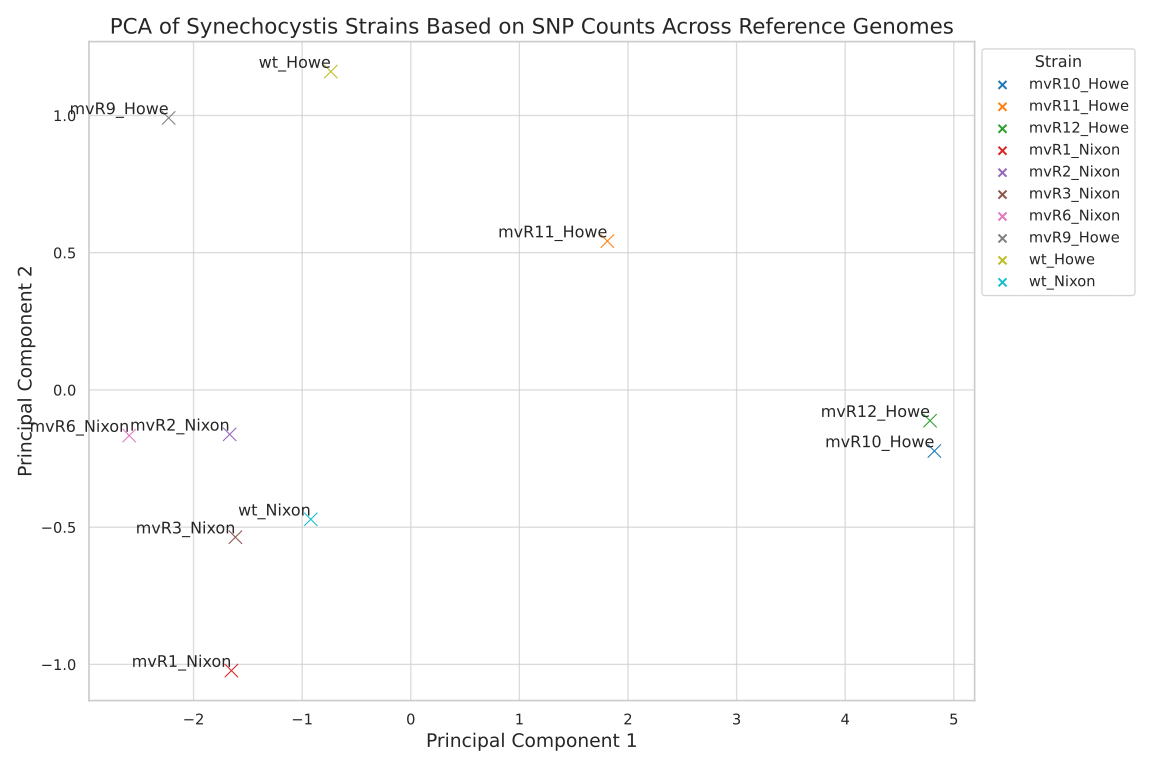
\includegraphics[width=\hsize]{../Figures/MV_adaptation/PCA_Synechocystis_Strains_SNP_Counts.png}
    \caption{Principal component analysis based on SNPs count of the sequenced genomes}
    \label{fig:PCA}
\end{figure}

Principal Component 1 (PC1) captured approximately 88.22\% of the total variance in the dataset. Principal Component 2 (PC2) accounted for about 5.37\% of the total variance. Cumulative Explained Variance: Together, the first two principal components capture approximately 93.58\% of the total variance. The first principal component (PC1) alone captures a significant proportion of the dataset's variance, indicating an effective reduction in dimensionality. The high cumulative explained variance (93.58\%) implies that the first two principal components provide a statistically robust representation of the dataset's original variability.
Therefore PCA analysis indicated that strains with the "Howe" and "Nixon" suffixes tend to cluster with their respective wild-types, corroborating the genomic closeness between mutants and their parental strains.

\subsection{SNPs Polimorphism}

\begin{figure}[H]
    \centering
    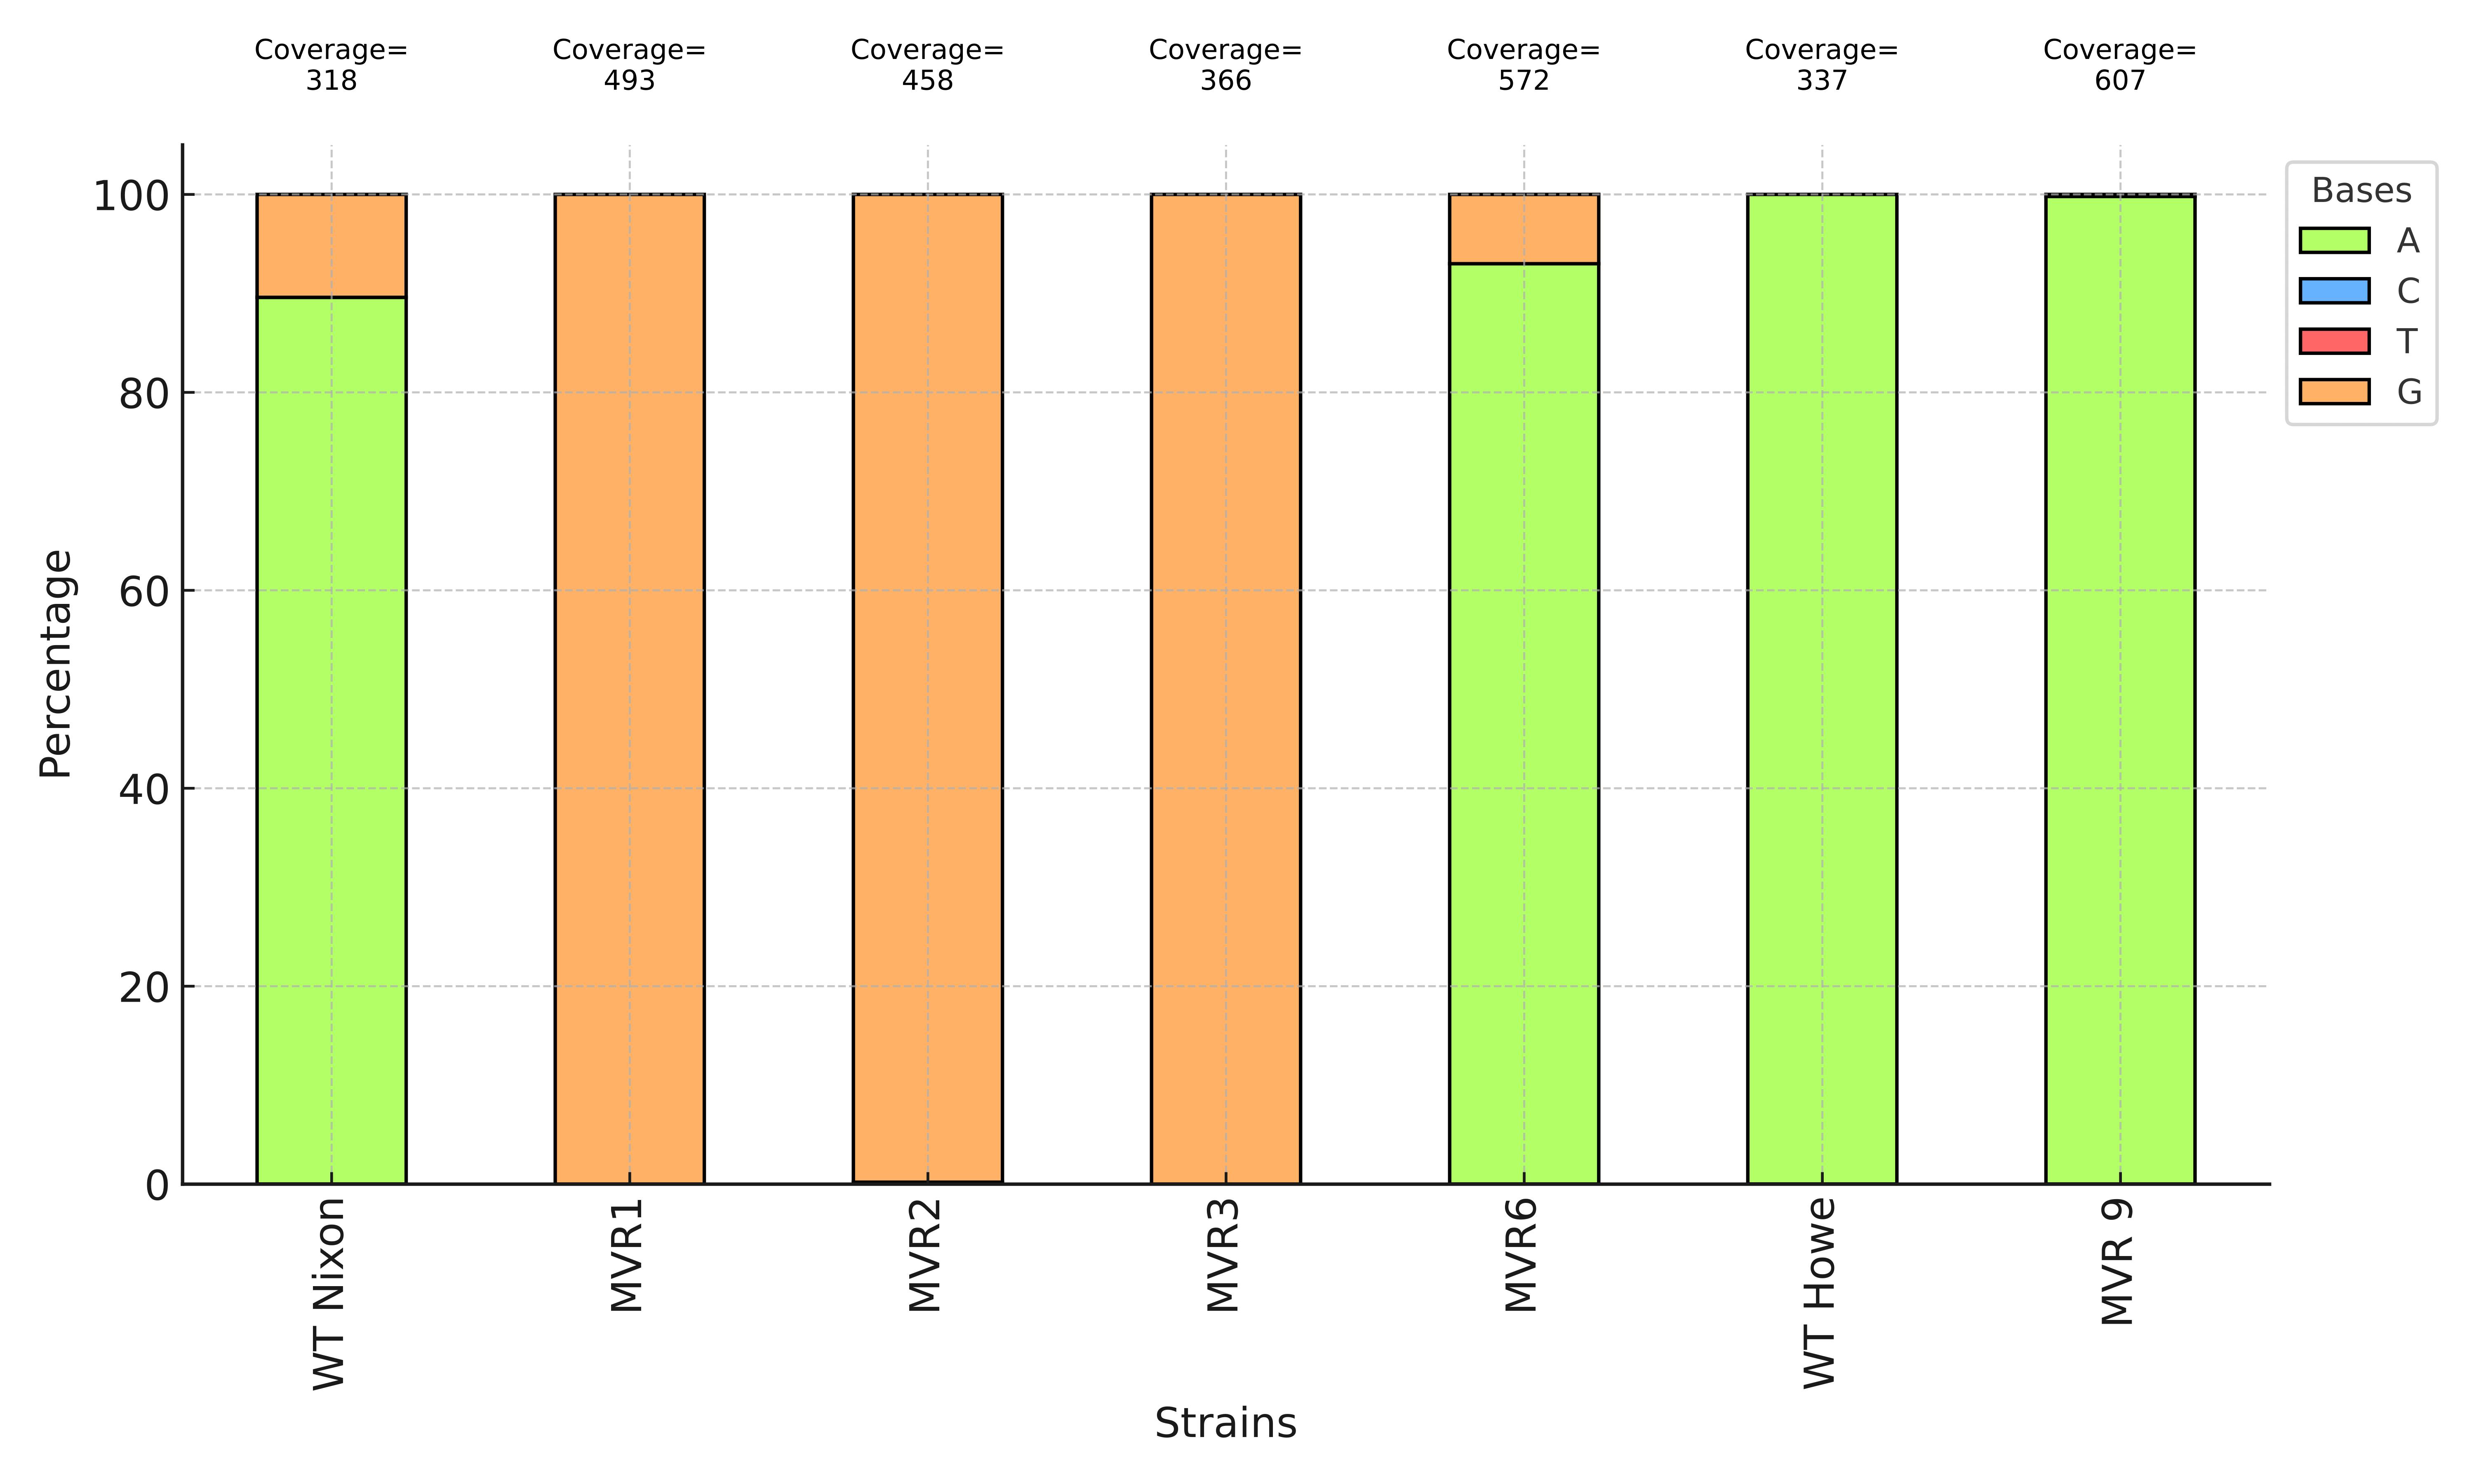
\includegraphics[width=\hsize]{../Figures/MV_adaptation/SNPolimorphism.png}
    \caption{Allelic frequency distribution of bases at the locus underlying the L139P mutation in sll1180 in wild-type and MV-resistant Synechocystis strains. The respective sequencing coverage for each strain is indicated above the bars. Bases are colour-coded as per the legend on the right}
    \label{fig:SNPS}
\end{figure}




\end{document}
